\documentclass[10pt,aspectratio=169]{ctexbeamer}

\usetheme{Madrid}
\usecolortheme{default}
\setbeamertemplate{navigation symbols}{}
\setbeamertemplate{footline}[frame number]

\usepackage{booktabs}
\usepackage{graphicx}
\usepackage{array}
\usepackage{tabularx}
\usepackage{amsmath}

\definecolor{PrimaryBlue}{HTML}{1E3A5F}
\definecolor{PrimaryTeal}{HTML}{0F766E}
\definecolor{AccentOrange}{HTML}{C26D2D}
\definecolor{AccentGray}{HTML}{64748B}
\definecolor{SoftGray}{HTML}{F3F6F9}

\setbeamercolor{title}{fg=PrimaryBlue}
\setbeamercolor{frametitle}{fg=PrimaryBlue}
\setbeamercolor{structure}{fg=PrimaryBlue}
\setbeamercolor{block title}{bg=PrimaryBlue!12,fg=PrimaryBlue}
\setbeamercolor{block body}{bg=SoftGray,fg=black}

\title{基于 NautilusTrader 的\\L2 订单簿本地持久化与专用结构优化}
\author{陈宝文}
\institute{中央财经大学}
\date{2026 年 3 月}

\newcommand{\decknote}[1]{\vspace{0.4em}{\scriptsize\color{AccentGray}#1}}

\newcommand{\assetorplaceholder}[2]{%
  \IfFileExists{#1}{%
    \includegraphics[width=\linewidth,height=0.58\textheight,keepaspectratio]{#1}%
  }{%
    \fcolorbox{AccentGray}{SoftGray}{%
      \begin{minipage}[c][0.52\textheight][c]{0.92\linewidth}
        \centering
        {\color{AccentGray}\large 占位图}\\[0.6em]
        {\footnotesize #2}\\[0.8em]
        {\scriptsize \texttt{\detokenize{#1}}}
      \end{minipage}
    }%
  }%
}

\begin{document}

\begin{frame}
  \titlepage
  \vspace{-0.8em}
  {\small
  研究主题：围绕 L2 订单簿的本地 research 效率优化，并为后续更真实的实盘接入做准备。}
\end{frame}

\begin{frame}{研究背景与意义}
  \begin{columns}[T]
    \begin{column}{0.55\textwidth}
      \begin{itemize}
        \item L2 订单簿数据更新频繁、体量大，本地回放成本高。
        \item 研究工作流会反复执行 replay、盘口查询和因子提取。
        \item 当前仍缺少成熟、面向 L2 特化并经过系统 workload 验证的开源优化实现。
        \item 因此，本课题希望在开源框架中建立一条可复现、可验证的 L2 优化路线。
      \end{itemize}
    \end{column}
    \begin{column}{0.45\textwidth}
      \assetorplaceholder{../assets/01_l2_research_motivation.png}{L2 research workflow concept}
    \end{column}
  \end{columns}
\end{frame}

\begin{frame}{问题定义与研究目标}
  \begin{columns}[T]
    \begin{column}{0.57\textwidth}
      \begin{block}{研究对象}
        面向 \texttt{L2 MBP} 订单簿，以原始交易所 delta 作为 source of truth。
      \end{block}
      \begin{itemize}
        \item 当前目标：提高本地 replay、query 与 research 的效率。
        \item 评价方式：统一 correctness 规则 + microbench + 真实 replay workload。
        \item 长期目标：将优化后的 L2 路径扩展到更真实的 live trading 场景。
      \end{itemize}
    \end{column}
    \begin{column}{0.43\textwidth}
      \assetorplaceholder{../assets/02_problem_scope.png}{scope and future integration}
    \end{column}
  \end{columns}
\end{frame}

\begin{frame}{Baseline 系统与开销来源}
  \begin{itemize}
    \item 选择 \texttt{nautilus\_trader} 作为 baseline 与后续集成载体。
    \item 其现有路径强调通用性，但在 L2 场景下仍保留了部分非必要抽象。
    \item 因此，本课题先不直接“换结构”，而是先回答：哪些 overhead 值得被削减？
  \end{itemize}
  \vspace{0.6em}
  \begin{block}{Baseline 路径概述}
    原始 L2 delta $\rightarrow$ 通用订单簿入口 $\rightarrow$ synthetic order 语义处理
    $\rightarrow$ ladder / level 容器 $\rightarrow$ 最终盘口状态
  \end{block}
  \vspace{0.4em}
  \begin{tabularx}{\linewidth}{>{\raggedright\arraybackslash}p{0.34\linewidth} >{\raggedright\arraybackslash}X}
    \toprule
    开销项 & 直观影响 \\
    \midrule
    synthetic order 语义 & 引入额外映射和 L2 不必要的路径复杂度 \\
    level 容器间接层 & 更新路径更长，内存对象和容器负担更重 \\
    额外 cache 维护 & 在 L2 场景中形成额外常数开销 \\
    通用路径分支 & 难以完全贴合 price level 导向的 L2 语义 \\
    \bottomrule
  \end{tabularx}
\end{frame}

\begin{frame}{研究方法：从 Overhead 到证据}
  \begin{columns}[T]
    \begin{column}{0.44\textwidth}
      \assetorplaceholder{../assets/04_overhead_method.png}{overhead to evidence}
    \end{column}
    \begin{column}{0.56\textwidth}
      \begin{enumerate}
        \item 建模 baseline 路径并识别主要 overhead。
        \item 设计不同数据结构，明确预期收益与 trade-off。
        \item 用统一 correctness 规则验证实现是否等价。
        \item 用 microbench 和 replay workload 检查预期是否成立。
      \end{enumerate}
      \vspace{0.6em}
      \begin{block}{统一分析模板}
        \textbf{目标 overhead} $\rightarrow$ \textbf{结构选型} $\rightarrow$ \textbf{trade-off} $\rightarrow$ \textbf{实验验证}
      \end{block}
    \end{column}
  \end{columns}
\end{frame}

\begin{frame}{技术路线总览}
  \begin{columns}[T]
    \begin{column}{0.48\textwidth}
      \assetorplaceholder{../assets/05_technical_roadmap.png}{Baseline to Tree, Vec, Grid}
    \end{column}
    \begin{column}{0.52\textwidth}
      \begin{itemize}
        \item \textbf{Baseline}：原生通用 L2 路径
        \item \textbf{L2TreeBook}：保留有序树，去除 L2 不必要抽象
        \item \textbf{L2VecBook}：强调连续内存与 query locality
        \item \textbf{L2GridBook}：利用 tick 离散化与 best pointer
      \end{itemize}
      \decknote{这不是一次性重写，而是一条循序渐进的优化路线。}
    \end{column}
  \end{columns}
\end{frame}

\begin{frame}{Phase 1：L2TreeBook}
  \begin{columns}[T]
    \begin{column}{0.44\textwidth}
      \assetorplaceholder{../assets/06_l2treebook_diagram.png}{L2TreeBook structure}
    \end{column}
    \begin{column}{0.56\textwidth}
      \begin{block}{目标 overhead}
        synthetic order 语义、per-level order 容器、额外 cache 维护
      \end{block}
      \begin{block}{trade-off}
        仍保留树结构，因此不是最激进的布局优化方案
      \end{block}
      \begin{block}{阶段结果}
        \begin{itemize}
          \item 纯 replay 吞吐相对 baseline 提升约 \textbf{28.7\%}
          \item 纯 replay 耗时下降约 \textbf{22\%}
          \item 峰值 RSS 从约 \textbf{51 MB} 降至约 \textbf{31.5 MB}
        \end{itemize}
      \end{block}
    \end{column}
  \end{columns}
\end{frame}

\begin{frame}{Phase 2：L2VecBook}
  \begin{columns}[T]
    \begin{column}{0.44\textwidth}
      \assetorplaceholder{../assets/07_l2vecbook_diagram.png}{L2VecBook structure}
    \end{column}
    \begin{column}{0.56\textwidth}
      \begin{block}{目标 overhead}
        改善 top-N 与 best-price 查询的内存连续性和 locality
      \end{block}
      \begin{block}{trade-off}
        中间价位插入和删除需要移动后续元素
      \end{block}
      \begin{block}{阶段结果}
        \begin{itemize}
          \item \texttt{best\_bid\_ask} 与 \texttt{top\_10\_query} microbench 最强
          \item 但真实 replay 吞吐仅约 \textbf{126k--127k updates/s}
          \item 说明连续布局优势被高频结构更新的搬移成本抵消
        \end{itemize}
      \end{block}
    \end{column}
  \end{columns}
\end{frame}

\begin{frame}{Phase 3：L2GridBook}
  \begin{columns}[T]
    \begin{column}{0.44\textwidth}
      \assetorplaceholder{../assets/08_l2gridbook_diagram.png}{L2GridBook structure}
    \end{column}
    \begin{column}{0.56\textwidth}
      \begin{block}{目标 overhead}
        减少部分树遍历与 price lookup 成本，利用 tick 离散化
      \end{block}
      \begin{block}{trade-off}
        page 分配、bitmap 维护与 best pointer 修复更复杂
      \end{block}
      \begin{block}{阶段结果}
        \begin{itemize}
          \item 真正的 chunked sparse grid 原型已经落地
          \item 但当前 replay 吞吐约 \textbf{181k--182k updates/s}，低于 \texttt{L2TreeBook}
          \item 峰值 RSS 约 \textbf{249 MB}，暴露了 sparse page 浪费与参数调优问题
        \end{itemize}
      \end{block}
    \end{column}
  \end{columns}
\end{frame}

\begin{frame}{实验设计与公平性}
  \begin{itemize}
    \item 同一数据集：\texttt{binance-futures\_incremental\_book\_L2\_2024-12-10\_BTCUSDT.csv.gz}
    \item 同一 replay 上限：\textbf{10,000,000} 条 delta
    \item 同一 workload：\texttt{replay\_only}、\texttt{q=100}、\texttt{q=1000}
    \item 同一深度配置：\textbf{depth=10}
    \item 同一 correctness 规则：best bid/ask、top-N、最终状态一致
  \end{itemize}
  \vspace{0.8em}
  \begin{block}{为什么这样的实验设计重要}
    只有在输入、workload 和 correctness 都固定的前提下，才能把性能差异归因到数据结构本身，而不是归因到环境差异或测试方式差异。
  \end{block}
\end{frame}

\begin{frame}{真实 workload：Replay 吞吐对比}
  \centering
  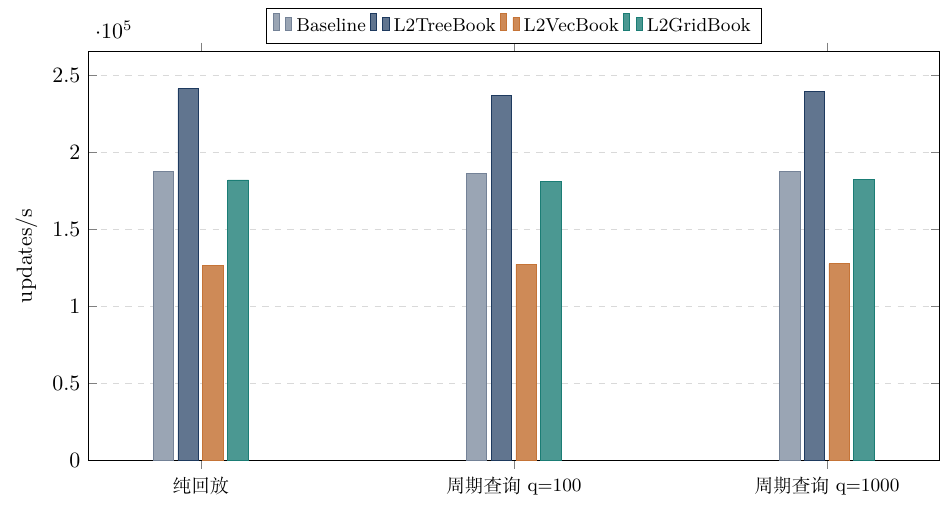
\includegraphics[width=\linewidth,height=0.72\textheight,keepaspectratio]{../assets/09_replay_throughput.png}
  \decknote{L2 专用语义已经显著提高 research 场景下的 replay 效率，其中 L2TreeBook 当前是最强实现；新的 L2GridBook 则揭示了非树型 grid 结构的真实 trade-off。}
\end{frame}

\begin{frame}{微基准与内存结果}
  \begin{columns}[T]
    \begin{column}{0.58\textwidth}
      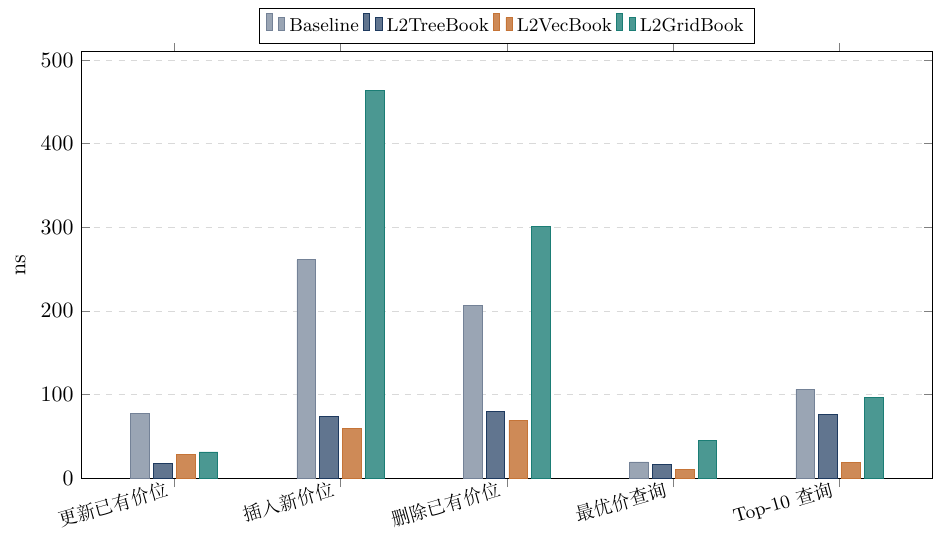
\includegraphics[width=\linewidth,height=0.62\textheight,keepaspectratio]{../assets/10_microbench.png}
    \end{column}
    \begin{column}{0.42\textwidth}
      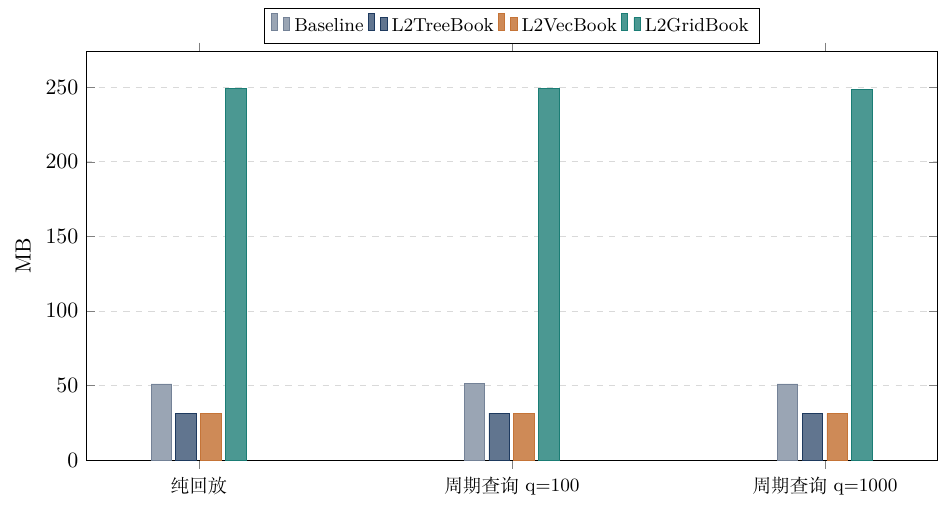
\includegraphics[width=\linewidth,height=0.62\textheight,keepaspectratio]{../assets/11_peak_rss.png}
    \end{column}
  \end{columns}
  \decknote{L2VecBook 在 query microbench 上优势明显，但真实 replay 较弱；新的 chunked L2GridBook 说明如果 page 过于稀疏，内存和插删常数都会明显恶化。}
\end{frame}

\begin{frame}{当前价值、风险与下一步}
  \begin{columns}[T]
    \begin{column}{0.56\textwidth}
      \begin{block}{当前价值}
        \begin{itemize}
          \item 已显著提高本地 replay 与 research 效率
          \item 已建立可复现的 workload、benchmark 与 correctness 框架
          \item 已较清楚地识别不同结构各自削减了什么 overhead，以及付出了什么代价
        \end{itemize}
      \end{block}
      \begin{block}{下一步}
        \begin{itemize}
          \item 继续优化 \texttt{L2GridBook} 的稳定性
          \item 完善中文图表与论文实验章节
          \item 研究如何把优化后的 L2 路径接到更真实的 live workflow
        \end{itemize}
      \end{block}
    \end{column}
    \begin{column}{0.44\textwidth}
      \assetorplaceholder{../assets/12_future_work.png}{future work roadmap}
    \end{column}
  \end{columns}
\end{frame}

\begin{frame}{谢谢}
  \centering
  \Large 感谢各位老师聆听，欢迎批评指正。\\[1.0em]
  \normalsize Questions and Discussion
\end{frame}

\end{document}
